\chapter{Desenvolvimento do projeto}

    O desenvolvimento do projeto foi dividido 
    em duas partes: a infraestrutura onde
    será tratado da parte física do projeto 
    necessária para o funcionamento 
    e o software que trata da parte de inteligencia
    do sistema e do histórico de variação de temperatura.

    De forma geral o funcionamento do projeto consiste
    como mostrado na figura \ref{fig:esquemaGeral}
    em sensores colocados em cada freezer e ligados 
    a um microcontrolador que estará conectado a internet
    e irá transmitir os dados de temperatura de cada 
    freezer para um servidor na nuvem, dados estes que poderão
    ser acessados através de um sistema web pelo computador
    ou um aplicativo (opcional) pelo celular.

    \begin{figure}[ht]
        \caption{Esquema Geral}
        \centering
        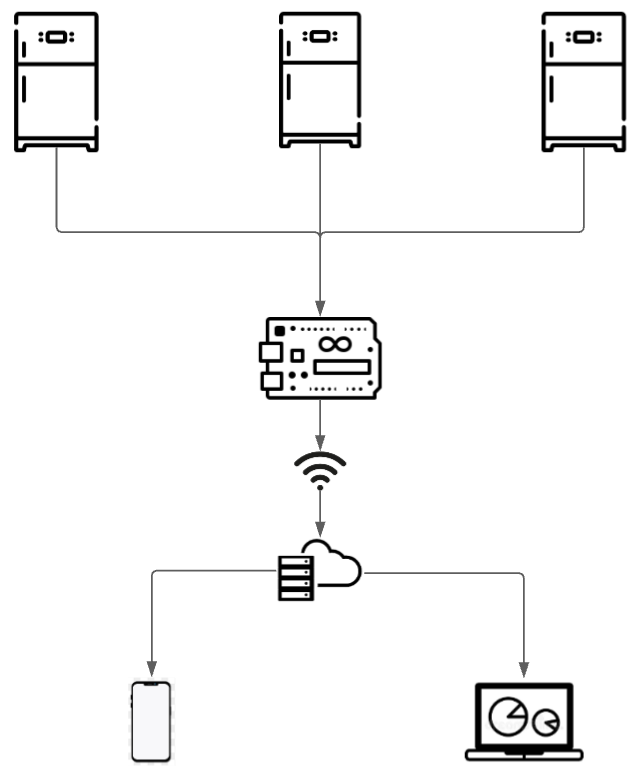
\includegraphics[width=0.5\textwidth]{img/esquema_geral.png}
        \legend{Fonte: Elaborado pelos autores}
        \label{fig:esquemaGeral}
    \end{figure}
